\section{Part (b)}
For each of the $105$ (15$\times$14/2) pairs of variables provided in "p1b.csv", repeat the steps in part (a) to compute the values of the test statistics as well as the p-values separately for: Mutual information, Jaccard Index and Pearson's chi-squared $\chi^2$ statistics. Select an $\alpha$ level to reject the null hypothesis of no association. For each of the three test statistics, determine the pairs with significant association at $\alpha$ level while adjusting for false discovery rate (see \textit{Note (3)} below). Draw scatter plots (or other appropriate visualizations) to compare the results of mutual information (MI), Jaccard Index (JI) and Pearson's chi-squared $\chi^2$. How much do the results of these three test statistics agree to one another? Which two of these three statistics are most similar (MI-JI, MI-$\chi^2$, or JI-$\chi^2$)? If you were to use only one of these three statistics, which one would you prefer to use and why? If you were to consider only your preferred test statistic among the given three, would your conclusions (about the associations of the provided variable pairs) change a lot? Make sure to specify the number of significantly associated pairs and the number of overlap between the three test statistics. Also, specify the selected $\alpha$ level and the number of permutations $N$ you use for the permutation tests.

\vspace{0.2cm}
\noindent
\textit{Note (3)}: Here, differently from part (a), we are testing for multiple hypotheses (one for each variable pair). Therefore, if we were to reject a null hypothesis as suggested in part (a) (when p-value is less than $\alpha$), we would have a considerably higher \href{https://en.wikipedia.org/wiki/False_discovery_rate}{false discovery rate (FDR)} than $\alpha$ (Think: If each test has a $\alpha$ chance of failure, what is the probability that there is at least one test that fails? For $\alpha = 0.05$ and $n=105$ tests, that would be $99.54\%$ chance of failure!). Thus, we need to use an appropriate procedure that take into account the number of hypotheses to make sure the FDR is indeed less than $\alpha$. For this purpose, you can apply one of the following two approaches: (1)~ \href{https://en.wikipedia.org/wiki/False_discovery_rate#Benjamini\%E2\%80\%93Hochberg_procedure}{Benjamini-Hochberg} procedure (which is, in many fields, the go-to way of adjusting for multiple hypotheses) to determine the statistically significant pairs, (2) A Monte Carlo simulation  specifically designed to control the FDR based on the distributions generated by the permutations (e.g., to compute the p-value of the top-scoring pair, we can use the distribution of the test statistics of the top-scoring pairs across all permutations, which would be a "multiple-hypthesis-corrected" null distribution).

\vspace{0.2cm}
\noindent
\textit{Note (4)}: Using the Benjamini-Hochberg procedure, essentially a stricter threshold is used to reject a null hypothesis (e.g., the threshold of $\dfrac{\alpha}{n}$ for rejecting the null hypothesis of the most significant pair). Therefore, for estimating the p-values using permutation test, you need to use more permutations compared to part (a) to be able find a significant association. Thus, make sure that your number of permutations $N$ is high enough to be able to find at least one significant pair.\\
-----\\

For the purpose of testing for multiple hypotheses and controlling for FDR, I applied the Benjamini-Hochberg (BH) procedure at $ \alpha = 0.05 $: to identify the most significant associations after FDR correction, we need enough permutations to reliably estimate p-values at about $ 0.05/105  \approx  0.0005 $; towards this end, I set $ N = 50,000 $.

Figure 5 gives the number of significant pairs detected by each statistic and Figure 6 gives the overlap between them:

\begin{center}
\begin{tabular}{|c|c|c|}
\hline
\textbf{Statistic} & \textbf{Significant Pairs} \\
\hline
Mutual Information & 91 \\
\hline
Jaccard Index & 56 \\
\hline
Pearson's $\chi^2$ & 90 \\
\hline
\end{tabular}
\end{center}

\begin{center}
\textbf{Figure 5:} Number of significant pairs detected by each statistic after Benjamini-Hochberg FDR correction at $\alpha = 0.05$.
\end{center}

\begin{center}
\begin{tabular}{|c|c|}
\hline
\textbf{Comparison} & \textbf{Number of Overlapping Pairs} \\
\hline
MI $\cap$ JI & 55 \\
\hline
MI $\cap$ $\chi^2$ & 89 \\
\hline
JI $\cap$ $\chi^2$ & 56 \\
\hline
MI $\cap$ JI $\cap$ $\chi^2$ & 55 \\
\hline
\end{tabular}
\end{center}

\begin{center}
\textbf{Figure 6:} Overlap of significant pairs between different statistics.
\end{center}

Below are the scatter plots side-by-side comparing each of the statistics:

\begin{center}
    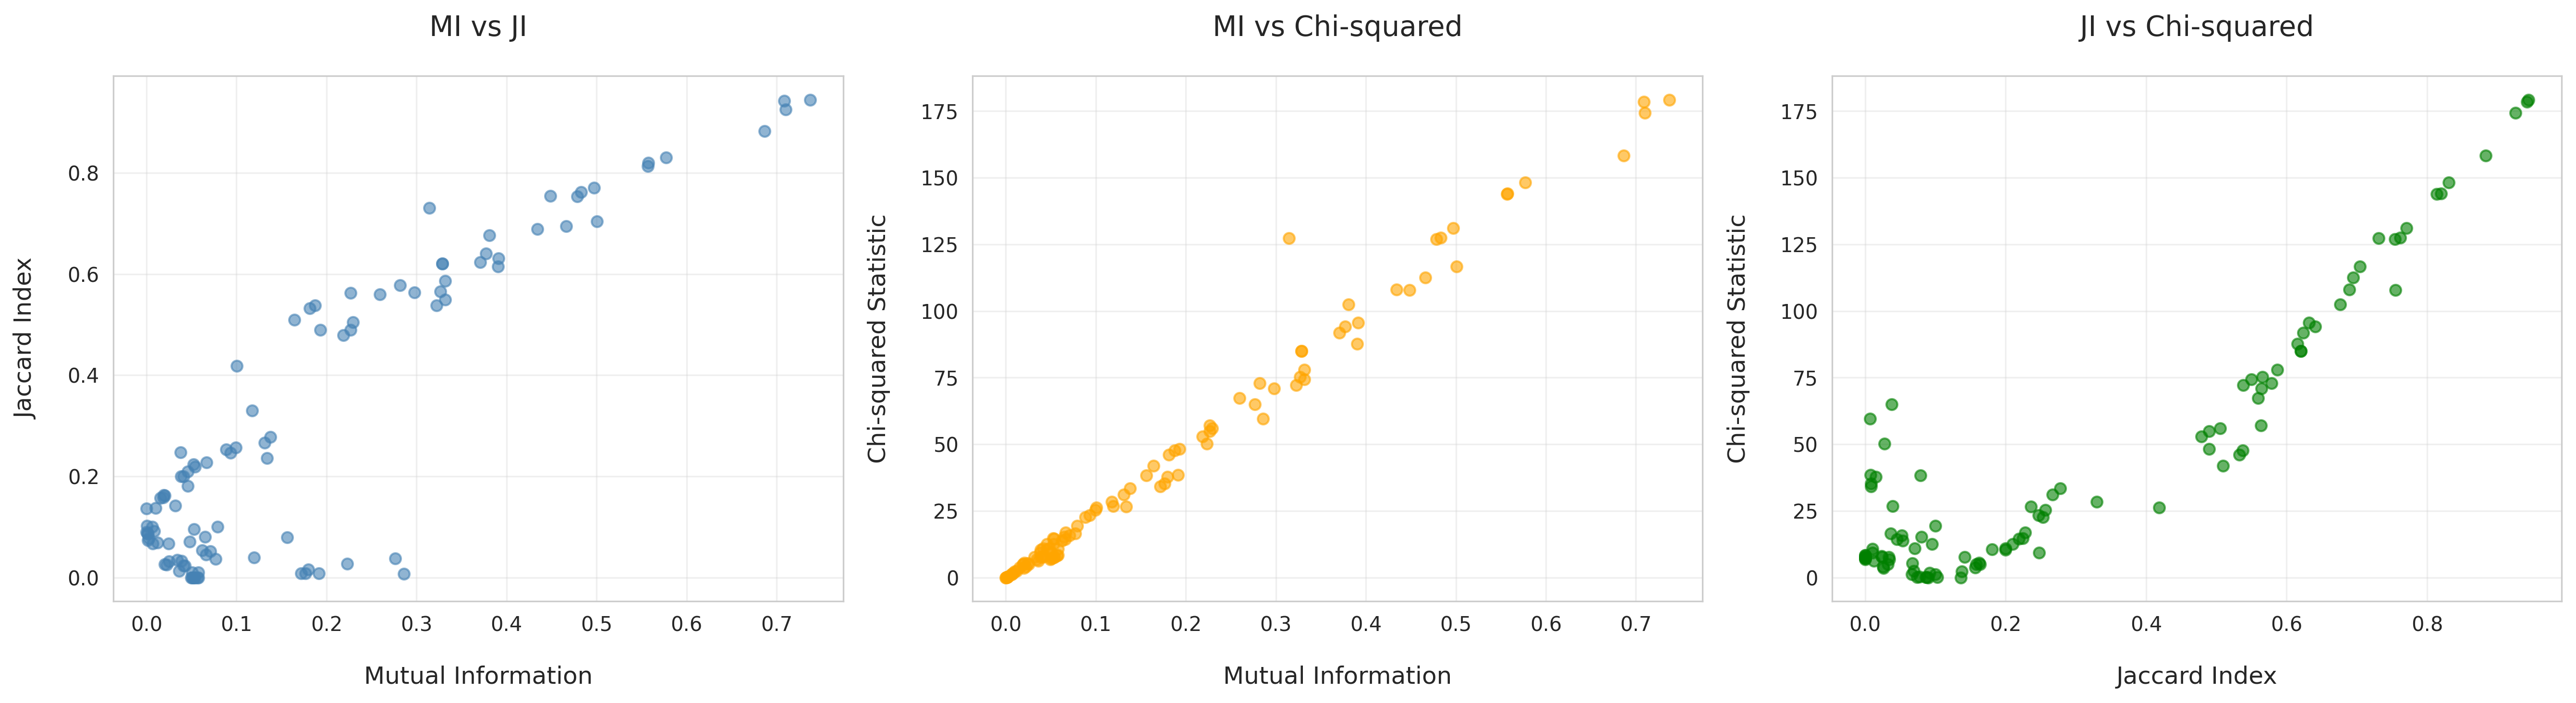
\includegraphics[width=0.95\textwidth]{figures/statistic_comparisons.png}
  
    \textbf{Figure 7:} Pairwise comparison of test statistics across 105 genomic variant pairs.
\end{center}

To characterize each pair from the visual: MI and chi-squared are very similar, showing a very high level of agreement. Jaccard relative to the other two show similar and moderate levels of agreement, but both show some level of difference at lower extremes.\\

Unsurprisingly from the discussion in the previous part, MI and chi-squared show a high degree of agreement while each agrees somewhat with Jaccard. Again, because both of these statistics use all four cells of the contingency table to represent deviation from independence, and Jaccard is constructed more as a similarity measure that is blind to the mutual exclusivity pattern in the data, their ability to identify associations in this data are both better than Jaccard and most similar to each other.\\

I would say that using either MI or Pearson's chi-squared is going to generally arrive at the same result; the only case where just using one statistic would get you very different conclusion would be Jaccard. However, the computationally efficiency of using chi-squared and not having to do many permutation tests to get essentially the same result would make it my preferred statistic. I think the difference in significant pairs by one may be more telling with additional exercises, but its not compelling enough given this test to believe that MI is noticeably superior.\\

\newpage
